% Created 2026-10-27 Tue 14:24
% Intended LaTeX compiler: pdflatex
\documentclass[11pt]{article}

\usepackage[utf8]{inputenc}
\usepackage[T1]{fontenc}
\usepackage{graphicx}
\usepackage{longtable}
\usepackage{wrapfig}
\usepackage{rotating}
\usepackage[normalem]{ulem}
\usepackage{amsmath}
\usepackage{amssymb}
\usepackage{capt-of}
\usepackage{hyperref}
\usepackage{minted}
\usepackage{tabularx}
\usepackage[inkscapelatex=false]{svg}
\usepackage[margin=0.25in]{geometry}
\usepackage{caption}
\usepackage{subcaption}
\usepackage{tikz}
\usepackage{booktabs}
\definecolor{bg}{rgb}{0.95,0.95,0.95}
\usepackage{underscore}
\setminted{linenos=true, numbersep=5pt}
\setcounter{secnumdepth}{2}
\author{Max Morabito}
\date{\today}
\title{Light Game Engine Quality Management Plan\\\medskip
\large Phase 1: Specification Based Testing}
\hypersetup{
 pdfauthor={Max Morabito},
 pdftitle={Light Game Engine Quality Management Plan},
 pdfkeywords={},
 pdfsubject={},
 pdfcreator={},
 pdflang={English}}
\begin{document}

\maketitle
\setcounter{tocdepth}{2}
\tableofcontents

\clearpage
\section{Project}
\label{sec:orgfe8fe27}

\subsection{Light}
\label{sec:org16fccec}
Light is a minimalist game engine, designed to allow a modern, editor-based workflow while being lightweight enough to run on the vast majority of modern hardware.  It was written over a period of about 20 days for CSC455 at SUNY Oswego.
It is available, fully open-source and free to use, at \url{https://github.com/vasuki1129/light}.


\begin{figure}[htbp]
  \centering
  \begin{subfigure}{0.80\textwidth}
  \centering
  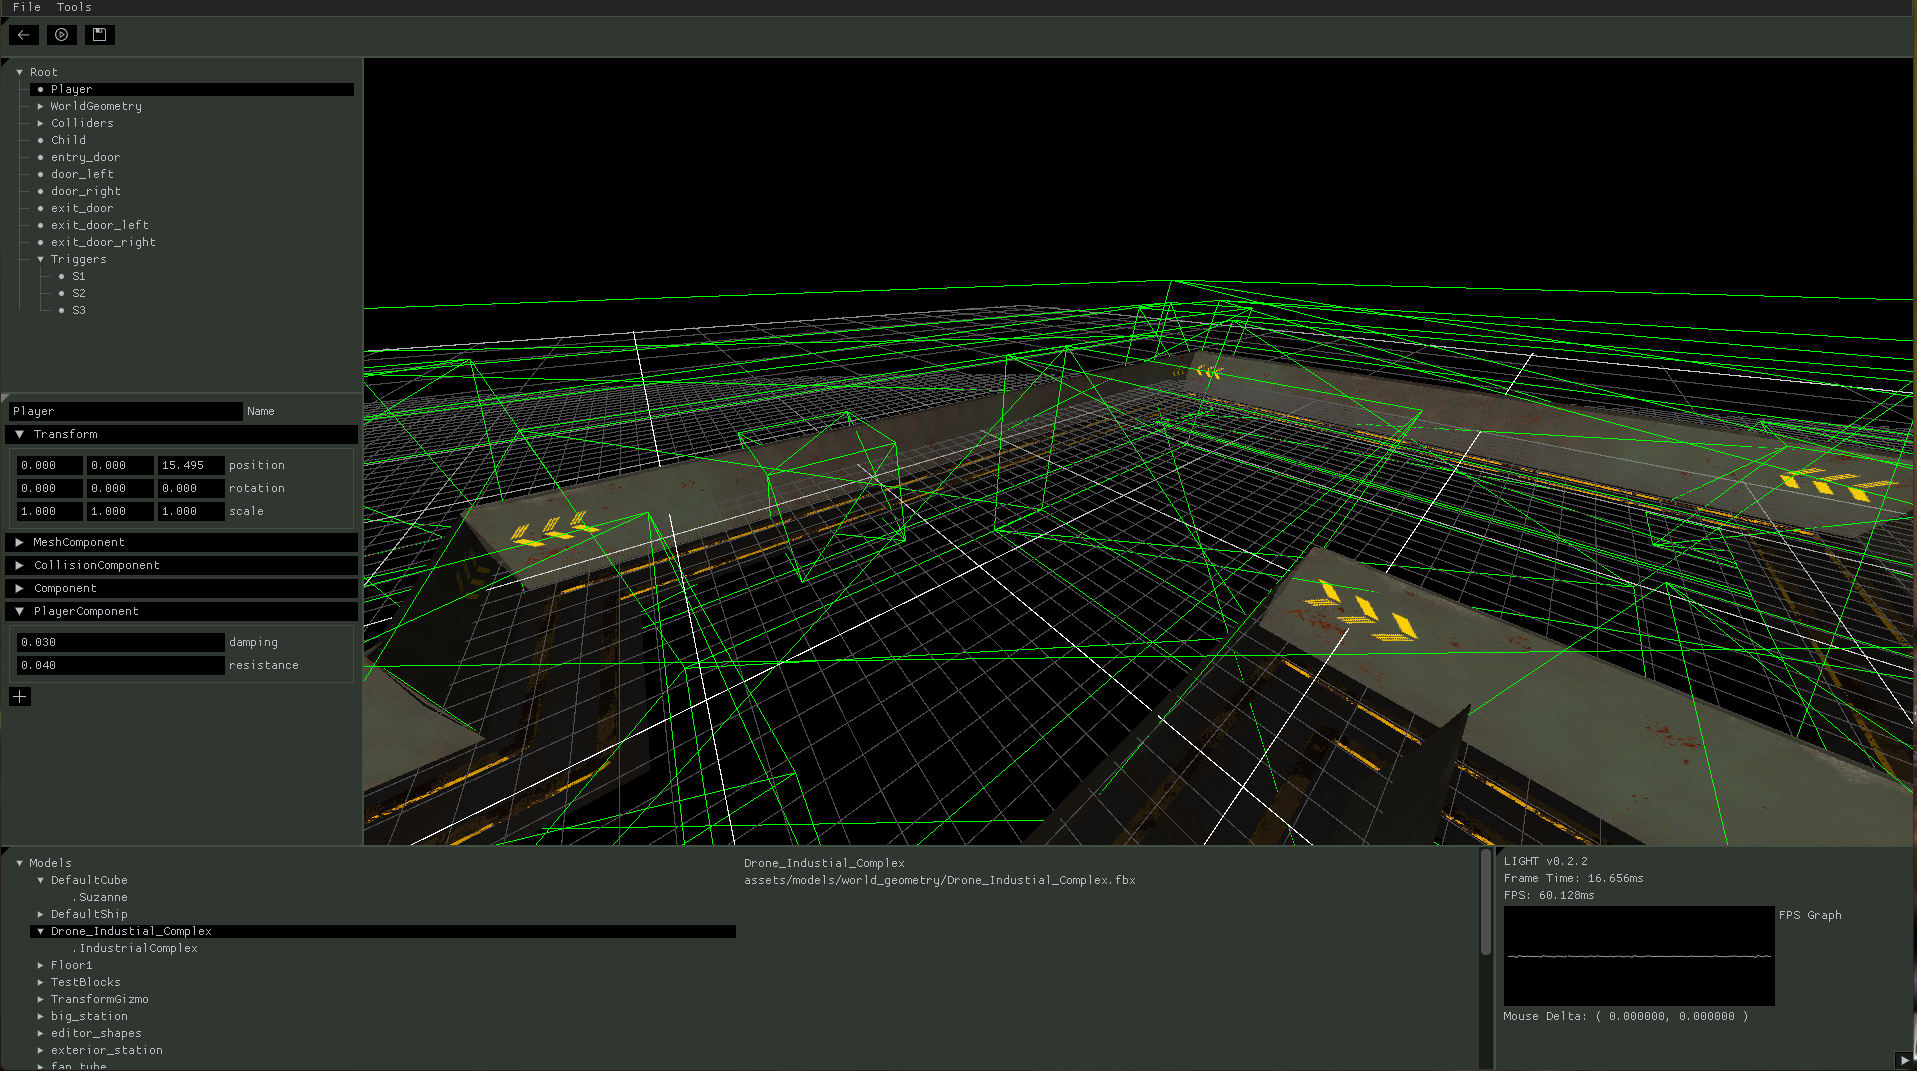
\includegraphics[width=0.98\textwidth]{diagrams/light_editor_ss}
  \caption{The engine in editor mode, being used to construct a scene.}
  \end{subfigure}
\end{figure}
\begin{figure}[htbp]
  \centering
  \begin{subfigure}{0.80\textwidth}
  \centering
  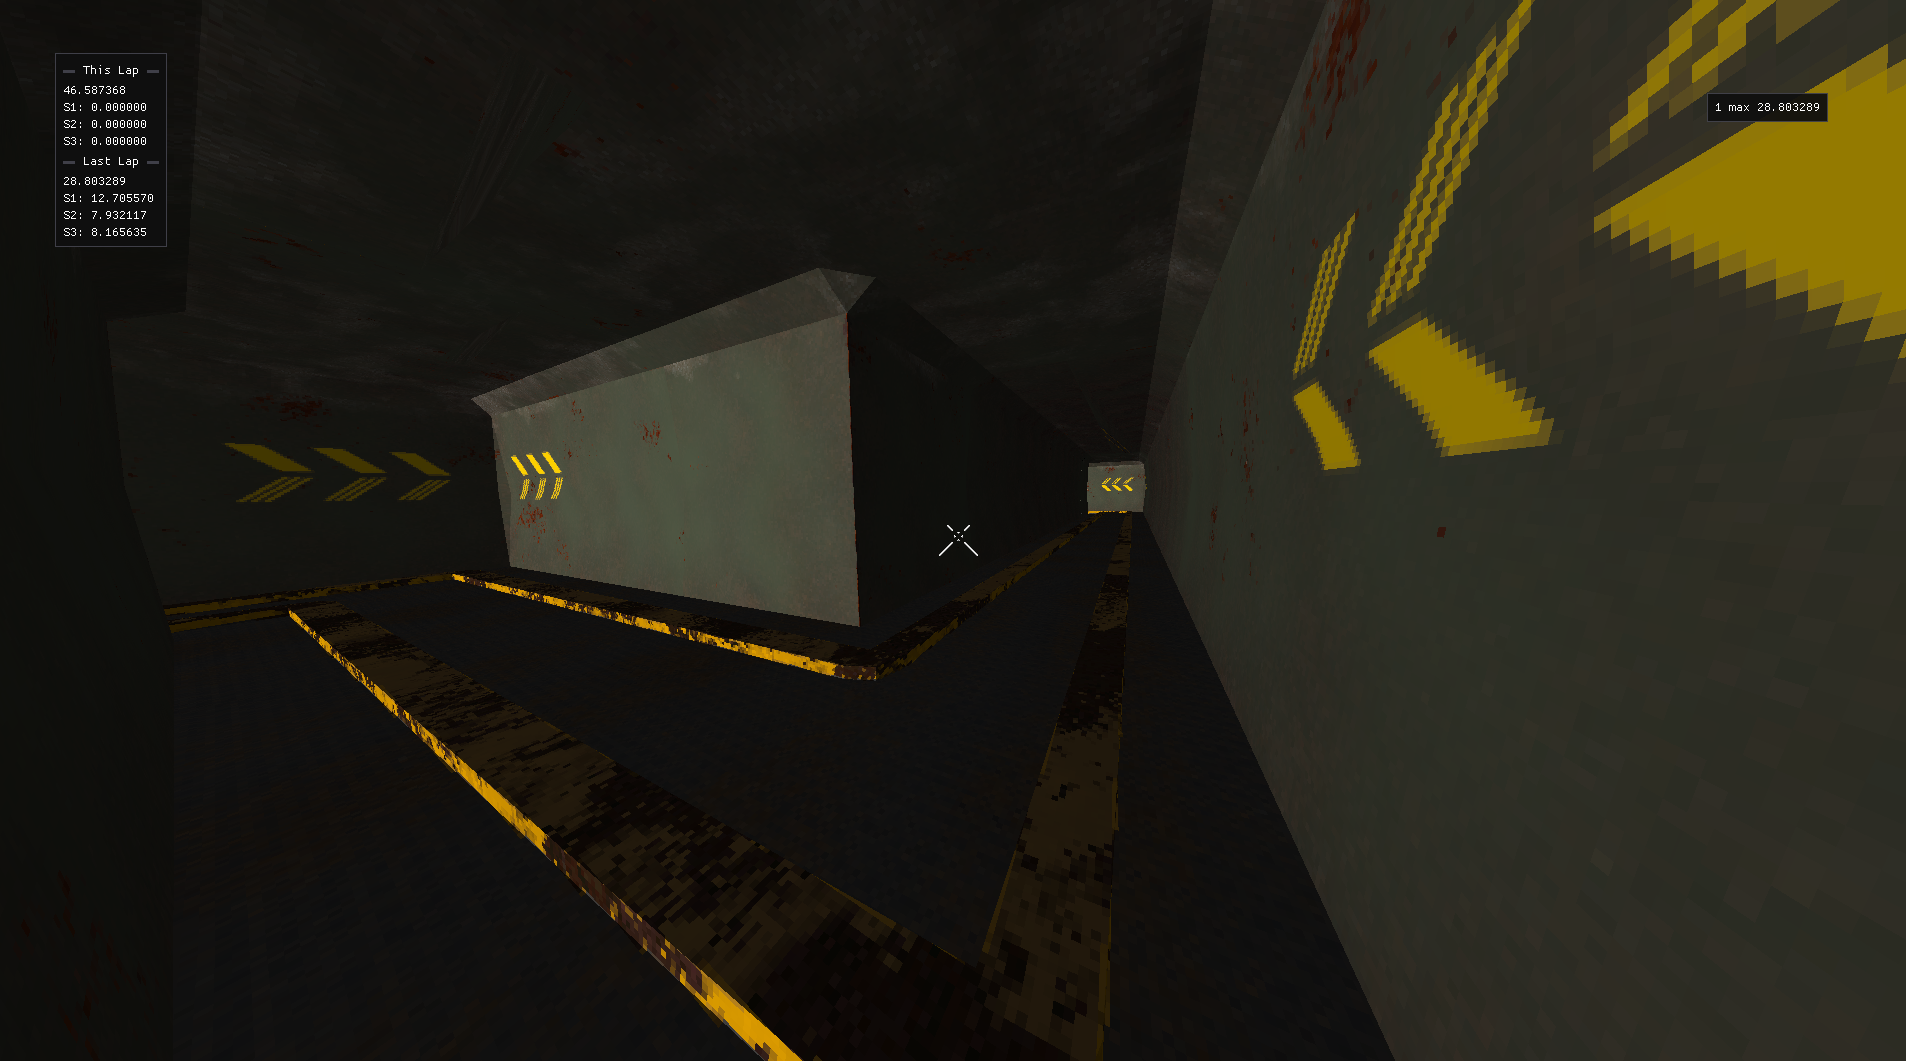
\includegraphics[width=0.98\textwidth]{diagrams/light_game_ss}
  \caption{The same scene in gameplay mode.}
  \end{subfigure}
\end{figure}

\clearpage
\subsection{Component Under Test}
\label{sec:orge4d5474}
The focus of the testing will be limited to the `Transform` class due to time constraints. This class is used to build a graph structure representing a 3D scene, along with allowing pieces of C++ code (`Component`s) to be attached to nodes in this graph.  The vast majority of the other features of the engine rely on this class, so it is the most critical to test.  Additionally, it is known to have at least one flaw.
\section{The Transform Class}
\label{sec:org45add83}
\subsection{Purpose}
\label{sec:org9a26bab}
The Transform class forms a single node in a rooted, directed graph that represents a three-dimensional scene.  Each transform represents the location, orientation, and scale of a coordinate frame (in mathematical terms, it defines a basis with an offset). The methods being tested here are the ones that allow constructing this graph, as well as the ones that interact with the Transform's spatial properties (position, rotation, and scale).
\subsection{Object Diagram}
\label{sec:org0fb072a}
This object diagram provides an example of what a transform graph might look like during a run of the program. Fields irrelevant to testing have been omitted.
\begin{center}
\includesvg[width=8cm]{diagrams/scenegraph_object_diagram}
\label{orgb5fcbfa}
\end{center}
\newpage
\subsection{Currently Known Flaw}
\label{sec:orge72f8a5}

To illustrate the flaw, imagine a transform called "A" at the origin, with a transform "B" as its child, translated along the Y axis an arbitrary distance.  If the transform "A" is rotated about its Z axis, the child should follow the parent, such that it maintains its position and rotation relative to the parent. Instead, the child rotates independently.

\begin{figure}[htbp]
  \centering
  \begin{subfigure}{0.30\textwidth}
  \centering
  \begin{tikzpicture}
    \node[draw] at (0,0) {A};
    \node[draw] at (0,3) {B};
  \end{tikzpicture}
  \caption{Initial setup, A is the parent of B}
  \end{subfigure}
  \hfill
  \begin{subfigure}{0.30\textwidth}
  \centering
  \begin{tikzpicture}
    \node[draw,rotate=-45] at (-3,0) {A};
    \node[draw,rotate=-45] at (-0.9,2.12) {B};
  \end{tikzpicture}
  \caption{Intended result after 45 degree clockwise rotation of A}
  \end{subfigure}
  \hfill
    \begin{subfigure}{0.30\textwidth}
  \centering
  
\begin{tikzpicture}
    \node[draw, rotate=-45] at (0,0) {A};
    \node[draw, rotate=-45] at (0,3) {B};
  \end{tikzpicture}
  \caption{Actual result with current code}
  \end{subfigure}
\end{figure}
\section{Quality Management Plan}
\label{sec:orgcd616cd}
\subsection{Quality Criteria}
\label{sec:org207065e}
\begin{center}
\begin{tabularx}{\textwidth}{lXXX}
\hline
\textbf{Quality Property} & \textbf{Definition} & \textbf{Metric} & \textbf{Criterion}\\
\hline
Functional Correctness & Test cases yield the expected results anticipated during derivation. & Number of test cases that pass. & 90\% of test cases pass.\\
\hline
Fault Tolerance & Software should run as intended even if invalid inputs are supplied. & Number of test cases that produce an unrecoverable error, such as a segfault. & All test cases properly recover from invalid inputs.\\
\hline
Performance & Software should run efficiently enough to allow smooth rendering. & Time taken to update state and render a frame. & Average frame time is under 16ms (60 frames per second or higher)\\
\hline
\end{tabularx}
\end{center}
\subsection{Quality Management Tools}
\label{sec:orgfa0ae68}
\begin{center}
\begin{tabularx}{\textwidth}{lXXX}
\hline
\textbf{Tool} & \textbf{Purpose}\\
\hline
Doxygen & Automatic generation of well-formatted documentation from source code comments.\\
\hline
Mermaid & Generation of control flow graphs from text definitions.\\
\hline
PlantUML & Generation of UML diagrams from text definition.\\
\hline
Doctest & Automated unit testing and result reporting.\\
\hline
\end{tabularx}
\end{center}
\subsection{Test Plan}
\label{sec:org89e2a61}
\begin{center}
\begin{tabularx}{\textwidth}{lXXX}
\hline
\textbf{Testing Phase} & \textbf{Testing Activity} & \textbf{Test Deadline}\\
\hline
Specification-Based Testing & Derivation of equivalence classes, boundary values, and test cases based on the specification of each method. & October 11th, 2026\\
\hline
\end{tabularx}
\end{center}

Further phases are yet to be determined.

\clearpage
\section{Equivalence Class Testing}
\label{sec:orgfa8ae60}

\subsection{Transform::AddChild(Transform* tr)}
\label{sec:org461bb10}
\subsubsection*{Specification}
\label{sec:org4a029fa}
\begin{minted}[frame=single,framerule=0.0mm,framesep=0mm,bgcolor=bg]{c++}
/**
 * Add a child transform to this transform
 *
 * If the desired child is already a child of this transform
 * log a warning and ignore it
 *
 * @param tr the transform to add as a child
 *
 */
void AddChild(Transform *tr);

\end{minted}
\subsubsection*{Equivalence Classes}
\label{sec:org2257289}
\begin{center}
\begin{tabularx}{\textwidth}{lXXX}
\hline
\textbf{Eq. Class ID} & \textbf{Param} & \textbf{Description} & \textbf{Representative}\\
\hline
4.1.EC1.1 & tr & a valid pointer & new Transform()\\
\hline
4.1.EC1.a & tr & a null pointer & nullptr\\
\hline
\end{tabularx}
\end{center}
\subsubsection*{Test Cases}
\label{sec:orgcd31f07}
\begin{center}
\begin{tabularx}{\textwidth}{lXXX}
\hline
\textbf{Test Case ID} & \textbf{Param.} & \textbf{Expected} & \textbf{Coverage}\\
 & \textit{tr} &  & \\
\hline
4.1.TC1 & A pointer to some valid Transform & No output & 4.1.EC1.1\\
\hline
4.1.TC2 & nullptr & Error: log message & 4.1.EC1.a\\
\hline
\end{tabularx}
\end{center}
\subsubsection*{Test Implementation}
\label{sec:org136d751}
\begin{minted}[frame=single,framerule=0.0mm,framesep=0mm,bgcolor=bg]{c++}
#include "../doctest/doctest.h"
#include "../engine/transform.h"
#include "../engine/component.h"
using namespace engine;

TEST_CASE("4.1.TC1") {
  Transform* test_transform = new Transform();
  Transform* child_transform = new Transform();
  //redirect cout to a string so we can check for the error message
  std::stringstream buffer;
  std::streambuf* old_cout = std::cout.rdbuf(buffer.rdbuf());
  test_transform->AddChild(child_transform);
  std::cout.rdbuf(old_cout);
  CHECK(buffer.str() == ""); //no output expected
}
TEST_CASE("4.1.TC2") {
  Transform* test_transform = new Transform();
  std::stringstream buffer;
  std::streambuf* old_cout = std::cout.rdbuf(buffer.rdbuf());
  test_transform->AddChild(nullptr);
  std::cout.rdbuf(old_cout);
  CHECK(buffer.str() != ""); //some kind of log output expected    
}
\end{minted}

\clearpage
\subsection{Transform::AddComponent(Component* component)}
\label{sec:orge9b6a3e}
\subsubsection*{Specification}
\label{sec:org6f8d233}
\begin{minted}[frame=single,framerule=0.0mm,framesep=0mm,bgcolor=bg]{c++}

/**
 * Add a component to this transform
 *
 * If the supplied pointer is null, log error and ignore
 * If the supplied pointer is not a component, log error and ignore
 *
 * @param component A pointer to the component to add
 */  
void AddComponent(Component* component);
\end{minted}
\subsubsection*{Equivalence Classes}
\label{sec:org132c0e8}
\begin{center}
\begin{tabularx}{\textwidth}{lXXX}
\hline
\textbf{Eq. Class ID} & \textbf{Param} & \textbf{Description} & \textbf{Representative}\\
\hline
4.2.EC1.1 & component & a valid pointer to a class that extends Component & new Component()\\
\hline
4.2.EC1.a & component & a valid pointer to something other than a Component & new Transform()\\
\hline
4.2.EC1.b & component & an invalid pointer & nullptr\\
\hline
\end{tabularx}
\end{center}
\subsubsection*{Test Cases}
\label{sec:orgeccc8d2}
\begin{center}
\begin{tabularx}{\textwidth}{lXXX}
\hline
\textbf{Test Case ID} & \textbf{Param.} & \textbf{Expected} & \textbf{Coverage}\\
 & \textit{tr} &  & \\
\hline
4.2.TC1 & new TestComponent() & No output & 4.2.EC1.1\\
\hline
4.2.TC2 & new Transform() & Disallowed by type checking, TC implementation omitted & 4.2.EC1.a\\
\hline
4.2.TC3 & nullptr & Error: log message and ignore & 4.2.EC1.b\\
\hline
\end{tabularx}
\end{center}
\subsubsection*{Test Implementation}
\label{sec:orgcaae13c}
\begin{minted}[frame=single,framerule=0.0mm,framesep=0mm,bgcolor=bg]{c++}
TEST_CASE("4.2.TC1") {
  Transform* test_transform = new Transform();
  Component* test_component = new Component();
  //redirect cout to a string so we can check for the error message
  std::stringstream buffer;
  std::streambuf* old_cout = std::cout.rdbuf(buffer.rdbuf());
  test_transform->AddComponent(test_component);
  std::cout.rdbuf(old_cout);
  CHECK(buffer.str() == ""); //no output expected
}
TEST_CASE("4.2.TC3") {
  Transform* test_transform = new Transform();
  Component* test_component = nullptr;
  std::stringstream buffer;
  std::streambuf* old_cout = std::cout.rdbuf(buffer.rdbuf());
  test_transform->AddComponent(test_component);
  std::cout.rdbuf(old_cout);
  CHECK(buffer.str() != ""); //some kind of log output expected
}
\end{minted}

\clearpage
\subsection{Transform::FindChildByName(std::string name)}
\label{sec:org142efcf}
\subsubsection*{Equivalence Classes}
\label{sec:org35ead83}
\begin{center}
\begin{tabularx}{\textwidth}{lXXX}
\hline
\textbf{Eq. Class ID} & \textbf{Param} & \textbf{Description} & \textbf{Representative}\\
\hline
4.3.EC1.1 & name & A string & "string"\\
\hline
4.3.EC1.2 & name & The empty string & ""\\
\hline
4.3.EC1.a & name & Not a string & 1\\
\hline
\end{tabularx}
\end{center}
\subsubsection*{Test Cases}
\label{sec:org5bffdef}
\begin{center}
\begin{tabularx}{\textwidth}{lXXX}
\hline
\textbf{Test Case ID} & \textbf{Param.} & \textbf{Expected} & \textbf{Coverage}\\
 & \textit{name} &  & \\
\hline
4.3.TC1 & "string" & nullptr & 4.3.EC1.1\\
\hline
4.3.TC2 & "" & nullptr & 4.3.EC1.2\\
\hline
4.3.TC3 & 1 & This will be disallowed by type checking, so TC implementation is omitted. & 4.3.EC1.a\\
\hline
\end{tabularx}
\end{center}

\begin{itemize}
\item The specification is unclear on whether the empty string is a valid name for a Transform, so I am assuming it is a valid transform name.
\end{itemize}
\subsubsection*{Test Implementation}
\label{sec:org73c59c9}
\begin{minted}[frame=single,framerule=0.0mm,framesep=0mm,bgcolor=bg]{c++}
TEST_CASE("4.3.TC1") {
  Transform* test_transform = new Transform();
  std::stringstream buffer;
  std::streambuf* old_cout = std::cout.rdbuf(buffer.rdbuf());
  Transform* out = test_transform->FindChildByName("string");
  std::cout.rdbuf(old_cout);
  CHECK(out == nullptr);
  delete test_transform;
}
TEST_CASE("4.3.TC2") {
  Transform* test_transform = new Transform();
  std::stringstream buffer;
  std::streambuf* old_cout = std::cout.rdbuf(buffer.rdbuf());
  Transform* out = test_transform->FindChildByName("");
  std::cout.rdbuf(old_cout);
  CHECK(out == nullptr);
  delete test_transform;
}
\end{minted}

\clearpage
\subsection{Transform::FindComponentByUID(uint64\textsubscript{t} id)}
\label{sec:org70a1028}

\subsubsection*{Equivalence Classes}
\label{sec:org4e52bae}
\begin{center}
\begin{tabularx}{\textwidth}{lXXX}
\hline
\textbf{Eq. Class ID} & \textbf{Param} & \textbf{Description} & \textbf{Representative}\\
\hline
4.4.EC1.1 & id & A positive integer & 1\\
\hline
4.4.EC1.2 & id & Zero & 0\\
\hline
4.4.EC1.a & id & A negative integer & -1\\
\hline
\end{tabularx}
\end{center}
\subsubsection*{Boundary Value Analysis}
\label{sec:org1e8b7e1}
\begin{center}
\begin{tabularx}{\textwidth}{lXXX}
\hline
Parameter & Boundary Values\\
\hline
id & 0, UINT64\textunderscore{}MAX\\
\hline
\end{tabularx}
\end{center}
\subsubsection*{Test Cases}
\label{sec:org0a377fe}
\begin{center}
\begin{tabularx}{\textwidth}{lXXX}
\hline
\textbf{Test Case ID} & \textbf{Param.} & \textbf{Expected} & Coverage\\
 & \textit{id} &  & \\
\hline
4.4.TC1 & 1 & nullptr & 4.4.EC1.1\\
\hline
4.4.TC2 & 0 & nullptr & 4.4.EC1.2\\
\hline
4.4.TC3 & -1 & Disallowed by type checking, TC implementation omitted & 4.4.EC1.a\\
\hline
\end{tabularx}
\end{center}

\textbf{Boundary Value Test Cases}
\begin{center}
\begin{tabularx}{\textwidth}{lXXX}
\hline
\textbf{Test Case ID} & \textbf{Param.} & \textbf{Expected} & Note\\
 & \textit{id} &  & \\
\hline
4.4.TC4 & 1 & nullptr & Already covered by 4.4.TC1\\
\hline
4.4.TC5 & 0 & nullptr & Already covered by 4.4.TC2\\
\hline
4.4.TC6 & -1 & Disallowed by type checking, TC implementation omitted & Already covered by 4.4.TC3\\
\hline
4.4.TC7 & UINT64\textunderscore{}MAX-1 & nullptr & \\
\hline
4.4.TC8 & UINT64\textunderscore{}MAX & nullptr & \\
\hline
4.4.TC9 & UINT64\textunderscore{}MAX+1 & same as 4.4.TC5 due to overflow & \\
\hline
\end{tabularx}
\end{center}

\clearpage
\subsubsection*{Test Implementation}
\label{sec:org3ace0c5}
\begin{minted}[frame=single,framerule=0.0mm,framesep=0mm,bgcolor=bg]{c++}
TEST_CASE("4.4.TC1") {
  Transform* test_transform = new Transform();
  Component* out = test_transform->FindComponentByUID(1);
  CHECK(out == nullptr);
  delete test_transform;
}
TEST_CASE("4.4.TC7") {
  Transform* test_transform = new Transform();
  Transform* out = test_transform->FindTransformByUID(UINT64_MAX-1);
  CHECK(out == nullptr);
  delete test_transform;
}
TEST_CASE("4.4.TC2") {
  Transform* test_transform = new Transform();
  Component* out = test_transform->FindComponentByUID(0);
  CHECK(out == nullptr);
  delete test_transform;
}
TEST_CASE("4.4.TC7") {
  Transform* test_transform = new Transform();
  Component* out = test_transform->FindComponentByUID(UINT64_MAX-1);
  CHECK(out == nullptr);
  delete test_transform;
}
TEST_CASE("4.4.TC8") {
  Transform* test_transform = new Transform();
  Component* out = test_transform->FindComponentByUID(UINT64_MAX);
  CHECK(out == nullptr);
  delete test_transform;
}
TEST_CASE("4.4.TC9") {
  Transform* test_transform = new Transform();
  Component* out = test_transform->FindComponentByUID(UINT64_MAX+1);
  CHECK(out == nullptr);
  delete test_transform;
}
\end{minted}

\clearpage
\subsection{Transform::FindTransformByUID(uint64\textsubscript{t} id)}
\label{sec:orgad73952}

\subsubsection*{Equivalence Classes}
\label{sec:orgae80899}
Equivalence classes same as Transform::FindComponentByUID.
\subsubsection*{Test Cases}
\label{sec:org531f2cb}
\begin{center}
\begin{tabularx}{\textwidth}{lXXX}
\hline
\textbf{Test Case ID} & \textbf{Param.} & \textbf{Expected} & Coverage\\
 & \textit{tr} &  & \\
\hline
4.5.TC1.1 & 1 & nullptr & 4.5.EC1.1\\
\hline
4.5.TC1.2 & 0 & nullptr & 4.5.EC1.2\\
\hline
4.5.TC1.a & -1 & Disallowed by type checking, TC implementation omitted & 4.5.EC1.a\\
\hline
\end{tabularx}
\end{center}
\subsubsection*{Boundary Value Analysis}
\label{sec:org5f5582e}
Boundary values and additional test cases are the same as 4.4.
\subsubsection*{Test Implementation}
\label{sec:org34a82f1}
\begin{minted}[frame=single,framerule=0.0mm,framesep=0mm,bgcolor=bg]{c++}
TEST_CASE("4.5.TC1") {
  Transform* test_transform = new Transform();
  Transform* out = test_transform->FindTransformByUID(1);
  CHECK(out == nullptr);
  delete test_transform;
}
TEST_CASE("4.5.TC2") {
  Transform* test_transform = new Transform();
  Transform* out = test_transform->FindTransformByUID(0);
  CHECK(out == nullptr);
  delete test_transform;
}
TEST_CASE("4.5.TC7") {
  Transform* test_transform = new Transform();
  Transform* out = test_transform->FindTransformByUID(UINT64_MAX-1);
  CHECK(out == nullptr);
  delete test_transform;
}
TEST_CASE("4.5.TC8") {
  Transform* test_transform = new Transform();
  Transform* out = test_transform->FindTransformByUID(UINT64_MAX);
  CHECK(out == nullptr);
  delete test_transform;
}
TEST_CASE("4.5.TC9") {
  Transform* test_transform = new Transform();
  Transform* out = test_transform->FindTransformByUID(UINT64_MAX+1);
  CHECK(out == nullptr);
  delete test_transform;
}

\end{minted}

\clearpage
\subsection{Transform::GetComponent(std::string name)}
\label{sec:org2bd916f}

\subsubsection*{Equivalence Classes}
\label{sec:orgf52b3b4}
Possible issues with specification:
\begin{itemize}
\item The method to get a transform by name is called `FindChildByName`, this method should be updated to match that scheme as `FindComponentByName`.

The equivalence classes are the same as Transform::FindChildByName.
\end{itemize}
\subsubsection*{Test Cases}
\label{sec:org8ae6c2b}

\begin{center}
\begin{tabularx}{\textwidth}{lXXX}
\hline
\textbf{Test Case ID} & \textbf{Param.} & \textbf{Expected} & \textbf{Coverage}\\
 & \textit{name} &  & \\
\hline
4.6.TC1 & "string" & nullptr & 4.6.EC1.1\\
\hline
4.6.TC2 & "" & nullptr & 4.6.EC1.2\\
\hline
4.6.TC3 & 1 & This will be disallowed by type checking, so TC implementation is omitted. & 4.6.EC1.a\\
\hline
\end{tabularx}
\end{center}
\subsubsection*{Test Implementation}
\label{sec:org8ac00ad}

\begin{minted}[frame=single,framerule=0.0mm,framesep=0mm,bgcolor=bg]{c++}
TEST_CASE("4.6.TC1") {
  Transform* test_transform = new Transform();
  Component* out = test_transform->GetComponent("string");
  CHECK(out == nullptr);
  delete test_transform;
}
TEST_CASE("4.6.TC2") {
  Transform* test_transform = new Transform();
  Component* out = test_transform->GetComponent("");
  CHECK(out == nullptr);
  delete test_transform;
}
\end{minted}

\clearpage
\subsection{Transform::GetGlobalPosition()}
\label{sec:org90ff586}
\subsubsection*{Equivalence Classes}
\label{sec:org672c477}
Takes no parameters, so equivalence class testing is not appropriate.
\subsection{Transform::GetGlobalRotation()}
\label{sec:org70d3b9b}
\subsubsection*{Equivalence Classes}
\label{sec:org78e4d7d}
Takes no parameters, so equivalence class testing is not appropriate.
\subsection{Transform::GetGlobalScale()}
\label{sec:org894f974}
\subsubsection*{Equivalence Classes}
\label{sec:orgd4ee8cc}
Takes no parameters, so equivalence class testing is not appropriate.

\clearpage
\subsection{Transform::Rotate(glm::vec3 axis, float amount)}
\label{sec:orgb983edf}
\subsubsection*{Equivalence Classes}
\label{sec:org4c9045e}
\begin{center}
\begin{tabularx}{\textwidth}{lXXX}
\hline
\textbf{Eq. Class ID} & \textbf{Param} & \textbf{Description} & \textbf{Representative}\\
\hline
4.10.EC1.1 & axis & axis is a vector with nonzero length & \{1.0,0.0,0.0\}\\
\hline
4.10.EC1.a & axis & axis is a vector with zero length & \{0.0,0.0,0.0\}\\
\hline
4.10.EC1.b & axis & axis is not a vector & 1\\
\hline
4.10.EC2.1 & amount & amount is a float & 90.0f\\
\hline
4.10.EC2.2 & amount & amount is an integer & 90\\
\hline
4.10.EC2.a & amount & amount is not a number & "90"\\
\hline
\end{tabularx}
\end{center}
\subsubsection*{Test Cases}
\label{sec:org30ec50c}
\begin{center}
\begin{tabularx}{\textwidth}{lXXXX}
\hline
\textbf{Test Case ID} & \textbf{Param.} &  & \textbf{Expected} & \textbf{Coverage}\\
 & \textit{axis} & \textit{amount} &  & \\
\hline
4.10.TC1 & \{1.0,0.0,0.0\} & 90.0f & No output & 4.10.EC1.1\\
 &  &  &  & 4.10.EC2.1\\
\hline
4.10.TC2 & \{1.0,0.0,0.0\} & 90 & No output & 4.10.EC2.2\\
\hline
4.10.TC3 & \{0.0,0.0,0.0\} & 90.0f & Error: log message & 4.10.EC1.a\\
\hline
4.10.TC4 & 1 & 90.0f & Disallowed by type checker & 4.10.EC1.b\\
\hline
4.10.TC5 & \{1.0,0.0,0.0\} & "90" & Disallowed by type checker & 4.10.EC2.a\\
\hline
\end{tabularx}
\end{center}
\subsubsection*{Test Implementation}
\label{sec:org28c5c74}

\begin{minted}[frame=single,framerule=0.0mm,framesep=0mm,bgcolor=bg]{c++}
TEST_CASE("4.10.TC1") {
  Transform* test_transform = new Transform();
  std::stringstream buffer;
  std::streambuf* old_cout = std::cout.rdbuf(buffer.rdbuf());
  test_transform->Rotate(glm::vec3(1.0,0.0,0.0), 90.0f);
  std::cout.rdbuf(old_cout);
  CHECK(buffer.str() == ""); //no output expected
  delete test_transform;
}
TEST_CASE("4.10.TC2") {
  Transform* test_transform = new Transform();
  std::stringstream buffer;
  std::streambuf* old_cout = std::cout.rdbuf(buffer.rdbuf());
  test_transform->Rotate(glm::vec3(1.0,0.0,0.0), 90);
  std::cout.rdbuf(old_cout);
  CHECK(buffer.str() == ""); //no output expected
  delete test_transform;
}
TEST_CASE("4.10.TC3") {
  Transform* test_transform = new Transform();
  std::stringstream buffer;
  std::streambuf* old_cout = std::cout.rdbuf(buffer.rdbuf());
  test_transform->Rotate(glm::vec3(0.0,0.0,0.0), 90.0f);
  std::cout.rdbuf(old_cout);
  CHECK(buffer.str() != ""); //Error log output expected
  delete test_transform;
}
\end{minted}

\clearpage
\subsection{Transform::Scale(glm::vec3 amount)}
\label{sec:orgf8fee8b}

\subsubsection*{Equivalence Classes}
\label{sec:org926f722}
\begin{center}
\begin{tabularx}{\textwidth}{lXXX}
\hline
\textbf{Eq. Class ID} & \textbf{Param} & \textbf{Description} & \textbf{Representative}\\
\hline
4.11.EC1.1 & amount & Any vector other than the zero vector or the identity vector of component-wise multiplication & \{x=2.0,y=3.0,z=2.0\}\\
\hline
4.11.EC1.2 & amount & The identity element of component-wise multiplication & \{x=1.0,y=1.0,z=1.0\}\\
\hline
4.11.EC1.3 & amount & The zero vector & \{x=0.0,y=0.0,z=0.0\}\\
\hline
4.11.EC1.a & amount & Not a vector & 1\\
\hline
\end{tabularx}
\end{center}
\subsubsection*{Test Cases}
\label{sec:org1816036}
\begin{center}
\begin{tabularx}{\textwidth}{lXXX}
\hline
\textbf{Test Case ID} & \textbf{Param.} & \textbf{Expected} & Coverage\\
 & \textit{amount} &  & \\
\hline
4.11.TC1 & \{2.0,3.0,2.0\} & No output & 4.11.EC1.1\\
\hline
4.11.TC2 & \{1.0,1.0,1.0\} & No output & 4.11.EC1.2\\
\hline
4.11.TC3 & \{0.0,0.0,0.0\} & No output & 4.11.EC1.3\\
\hline
4.11.TC4 & 1 & Disallowed by type checker & 4.11.EC1.a\\
\hline
\end{tabularx}
\end{center}
\subsubsection*{Test Implementation}
\label{sec:org8db361a}
\begin{minted}[frame=single,framerule=0.0mm,framesep=0mm,bgcolor=bg]{c++}
TEST_CASE("4.11.TC1") {
  Transform* test_transform = new Transform();
  glm::vec3 test_vector = glm::vec3(2.0,3.0,2.0);
  std::stringstream buffer;
  std::streambuf* old_cout = std::cout.rdbuf(buffer.rdbuf());
  test_transform->Scale(test_vector);
  std::cout.rdbuf(old_cout);
  CHECK(buffer.str() == ""); //no output expected
  delete test_transform;
}
TEST_CASE("4.11.TC2") {
  Transform* test_transform = new Transform();
  glm::vec3 test_vector = glm::vec3(1.0,1.0,1.0);
  std::stringstream buffer;
  std::streambuf* old_cout = std::cout.rdbuf(buffer.rdbuf());
  test_transform->Scale(test_vector);
  std::cout.rdbuf(old_cout);
  CHECK(buffer.str() == ""); //no output expected
  delete test_transform;
}
TEST_CASE("4.11.TC3") {
  Transform* test_transform = new Transform();
  glm::vec3 test_vector = glm::vec3(0.0,0.0,0.0);
  std::stringstream buffer;
  std::streambuf* old_cout = std::cout.rdbuf(buffer.rdbuf());
  test_transform->Scale(test_vector);
  std::cout.rdbuf(old_cout);
  CHECK(buffer.str() == ""); //no output expected
  delete test_transform;
}
\end{minted}

\clearpage
\subsection{Transform::Translate(glm::vec3 offset)}
\label{sec:org56d003c}

\subsubsection*{Equivalence Classes}
\label{sec:org476b5fd}
\begin{center}
\begin{tabularx}{\textwidth}{lXXX}
\hline
\textbf{Eq. Class ID} & \textbf{Param} & \textbf{Description} & \textbf{Representative}\\
\hline
4.12.EC1.1 & amount & Any vector that is not the identity vector & \{x=2.0,y=3.0,z=2.0\}\\
\hline
4.12.EC1.2 & amount & The identity vector for addition & \{x=0.0,y=0.0,z=0.0\}\\
\hline
4.12.EC1.a & amount & Not a vector & 1\\
\hline
\end{tabularx}
\end{center}
\subsubsection*{Test Cases}
\label{sec:orgc354406}
\begin{center}
\begin{tabularx}{\textwidth}{lXXX}
\hline
\textbf{Test Case ID} & \textbf{Param.} & \textbf{Expected} & Coverage\\
 & \textit{amount} &  & \\
\hline
4.12.TC1 & \{2.0,3.0,2.0\} & No output & 4.12.EC1.1\\
\hline
4.12.TC2 & \{0.0,0.0,0.0\} & No output & 4.12.EC1.2\\
\hline
4.12.TC3 & 1 & Disallowed by type checker & 4.12.EC1.a\\
\hline
\end{tabularx}
\end{center}
\subsubsection*{Test Implementation}
\label{sec:orgf11a9b0}
\begin{minted}[frame=single,framerule=0.0mm,framesep=0mm,bgcolor=bg]{c++}
TEST_CASE("4.12.TC1") {
  Transform* test_transform = new Transform();
  glm::vec3 test_vector = glm::vec3(2.0,3.0,2.0);
  std::stringstream buffer;
  std::streambuf* old_cout = std::cout.rdbuf(buffer.rdbuf());
  test_transform->Translate(test_vector);
  std::cout.rdbuf(old_cout);
  CHECK(buffer.str() == ""); //some kind of log output expected 
  delete test_transform;
}
TEST_CASE("4.12.TC2") {
  Transform* test_transform = new Transform();
  glm::vec3 test_vector = glm::vec3(0.0,0.0,0.0);
  std::stringstream buffer;
  std::streambuf* old_cout = std::cout.rdbuf(buffer.rdbuf());
  test_transform->Translate(test_vector);
  std::cout.rdbuf(old_cout);
  CHECK(buffer.str() == ""); //some kind of log output expected 
  delete test_transform;
}
\end{minted}

\clearpage
\section{Source Code Based Testing}
\label{sec:orgdc7ecfd}
\subsection{Transform::AddChild(Transform* tr)}
\label{sec:org9535a80}

\subsubsection*{Source Code}
\label{sec:org0618140}
\begin{minted}[frame=single,framerule=0.0mm,framesep=0mm,bgcolor=bg]{c++}
void Transform::AddChild(Transform *tr) {
  if (tr == nullptr) {
    std::cout << "Error: null transform passed to Transform::AddChild\n";
    return;
  }
  tr->parent = this;
  this->children.push_back(tr);
}
\end{minted}
\subsubsection*{Control Flow Graph}
\label{sec:orgf5ad76d}
\begin{center}
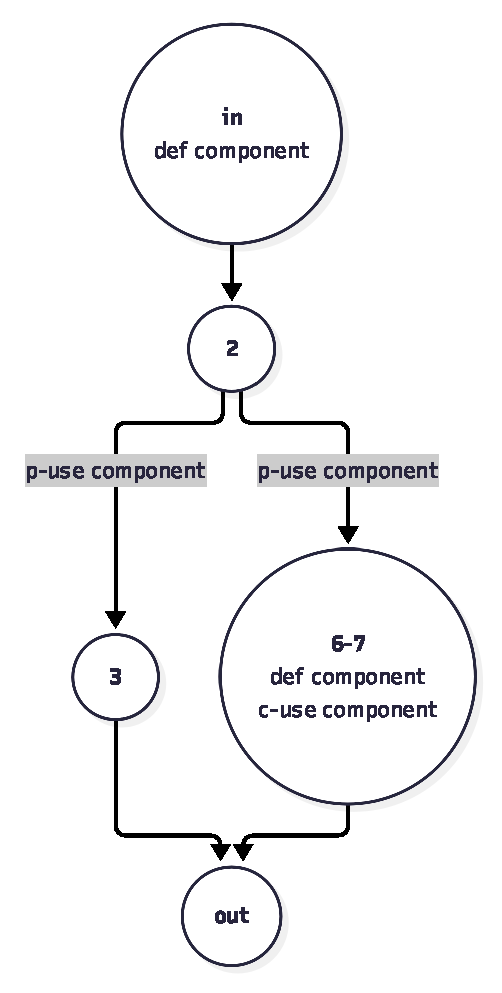
\includegraphics[width=8cm]{diagrams/transform/addchild.pdf}
\end{center}
\subsection{Transform::AddComponent(Component* component)}
\label{sec:orgabd0ca3}
\subsubsection*{Source Code}
\label{sec:orgea0b6e3}
\begin{minted}[frame=single,framerule=0.0mm,framesep=0mm,bgcolor=bg]{c++}
void Transform::AddComponent(Component *component) {
  if (component == nullptr)
  {
    std::cout << "Error: null component passed to Transform::AddComponent\n";
    return;
  }
  component->SetOwner(this);
  this->components.push_back(component);
}
\end{minted}
\subsubsection*{Control Flow Graph}
\label{sec:orgb768cc8}
\begin{center}
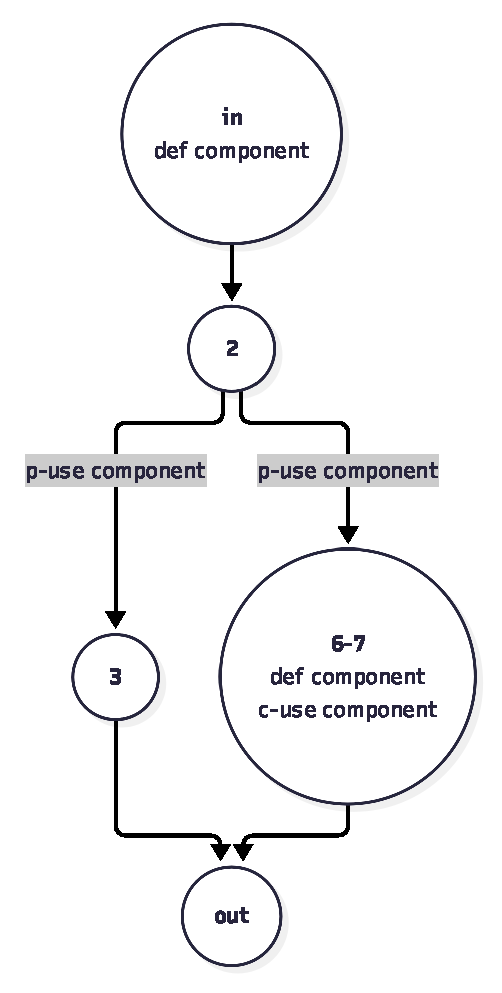
\includegraphics[width=8cm]{diagrams/transform/addchild.pdf}
\end{center}
\section{Test Results}
\label{sec:org7fdca99}

Running the suite of test cases described in this document yields the following output.

\begin{verbatim}
[doctest] doctest version is "2.5.0"
[doctest] run with "--help" for options
===============================================================================
[doctest] test cases: 27 | 27 passed | 0 failed | 0 skipped
[doctest] assertions: 27 | 27 passed | 0 failed |
[doctest] Status: SUCCESS!
\end{verbatim}

This indicates that the system is working as intended with regard to its handling of valid and invalid inputs.
\end{document}
